\documentclass{article}

\usepackage{fancyhdr}
\usepackage{extramarks}
\usepackage{amsmath}
\usepackage{amsthm}
\usepackage{amsfonts}
\usepackage{tikz}
\usepackage[plain]{algorithm}
\usepackage{algpseudocode}
\usepackage{enumerate}
\usepackage{tikz}
\usepackage{stfloats}
\usepackage{float}

\usetikzlibrary{automata,positioning}

%
% Basic Document Settings
%  

\topmargin=-0.45in
\evensidemargin=0in
\oddsidemargin=0in
\textwidth=6.5in
\textheight=9.0in
\headsep=0.25in

\linespread{1.1}

\pagestyle{fancy}
\lhead{\hmwkAuthorName}
\chead{\hmwkClass : \hmwkTitle}
\rhead{\firstxmark}
\lfoot{\lastxmark}
\cfoot{\thepage}

\renewcommand\headrulewidth{0.4pt}
\renewcommand\footrulewidth{0.4pt}

\setlength\parindent{0pt}

%
% Create Problem Sections
%

\newcommand{\enterProblemHeader}[1]{
    \nobreak\extramarks{}{Problem \arabic{#1} continued on next page\ldots}\nobreak{}
    \nobreak\extramarks{Problem \arabic{#1} (continued)}{Problem \arabic{#1} continued on next page\ldots}\nobreak{}
}

\newcommand{\exitProblemHeader}[1]{
    \nobreak\extramarks{Problem \arabic{#1} (continued)}{Problem \arabic{#1} continued on next page\ldots}\nobreak{}
    \stepcounter{#1}
    \nobreak\extramarks{Problem \arabic{#1}}{}\nobreak{}
}

\newcommand*\circled[1]{\tikz[baseline=(char.base)]{
		\node[shape=circle,draw,inner sep=2pt] (char) {#1};}}


\setcounter{secnumdepth}{0}
\newcounter{partCounter}
\newcounter{homeworkProblemCounter}
\setcounter{homeworkProblemCounter}{1}
\nobreak\extramarks{Problem \arabic{homeworkProblemCounter}}{}\nobreak{}

%
% Homework Problem Environment
%
% This environment takes an optional argument. When given, it will adjust the
% problem counter. This is useful for when the problems given for your
% assignment aren't sequential. See the last 3 problems of this template for an
% example.
%

\newenvironment{homeworkProblem}[1][-1]{
    \ifnum#1>0
        \setcounter{homeworkProblemCounter}{#1}
    \fi
    \section{Problem \arabic{homeworkProblemCounter}}
    \setcounter{partCounter}{1}
    \enterProblemHeader{homeworkProblemCounter}
}{
    \exitProblemHeader{homeworkProblemCounter}
}

%
% Homework Details
%   - Title
%   - Class
%   - Due date
%   - Name
%   - Student ID

\newcommand{\hmwkTitle}{Homework\ \#02}
\newcommand{\hmwkClass}{Probability \& Statistics for EECS}
\newcommand{\hmwkDueDate}{Feb 26, 2023}
\newcommand{\hmwkAuthorName}{Zhou Shouchen}
\newcommand{\hmwkAuthorID}{2021533042}


%
% Title Page
%

\title{
    \vspace{2in}
    \textmd{\textbf{\hmwkClass:\\  \hmwkTitle}}\\
    \normalsize\vspace{0.1in}\small{Due\ on\ \hmwkDueDate\ at 23:59}\\
	\vspace{4in}
}

\author{
	Name: \textbf{\hmwkAuthorName} \\
	Student ID: \hmwkAuthorID}
\date{}

\renewcommand{\part}[1]{\textbf{\large Part \Alph{partCounter}}\stepcounter{partCounter}\\}

%
% Various Helper Commands
%

% Useful for algorithms
\newcommand{\alg}[1]{\textsc{\bfseries \footnotesize #1}}
% For derivatives
\newcommand{\deriv}[1]{\frac{\mathrm{d}}{\mathrm{d}x} (#1)}
% For partial derivatives
\newcommand{\pderiv}[2]{\frac{\partial}{\partial #1} (#2)}
% Integral dx
\newcommand{\dx}{\mathrm{d}x}
% Alias for the Solution section header
\newcommand{\solution}{\textbf{\large Solution}}
% Probability commands: Expectation, Variance, Covariance, Bias
\newcommand{\E}{\mathrm{E}}
\newcommand{\Var}{\mathrm{Var}}
\newcommand{\Cov}{\mathrm{Cov}}
\newcommand{\Bias}{\mathrm{Bias}}

\begin{document}

\maketitle

\pagebreak

\begin{homeworkProblem}[1]

(a) Since $(a_1,a_2,\cdots,a_n)$ is no repetitions, so for any $a_i$, there are $n$ choices, and there are totally $n$ numbers in the sequence,
so the total number of possible bootstrap samples is $n^n$.\\

(b) Since that the order does not matter, and $(a_1,a_2,\cdots,a_n)$ is no repetitions, so we let $x_i$ be the 
times that $a_i$ has been chosen.\\
And $x_1 + x_2 + \cdots + x_n = n(x_i \geq 0)$, and all $x_i$ are integer.\\
From the Bose-Einstein Counting we have learned in class, we could know that 
there are total ${n+n-1\choose n-1}={2n-1\choose n-1}$ different ways.\\
So above all, there are ${2n-1\choose n-1}$ possible bootstrap samples.\\

(c) Since find an unordered bootstrap sample $\mathbf{b}_1$ is as likely as possible, 
so $\mathbf{b}_1$ is the sample that with $n$ distinct elements.\\
So $$p_1 = \dfrac{\#n\ different\ elements}{\# all\ possible\ choices}$$
$$= \dfrac{n!}{n^n}$$

Since find an unordered bootstrap sample $\mathbf{b}_2$ is as unlikely as possible, 
so $\mathbf{b}_2$ is the sample that with all elements are the same unique element.\\
So $$p_2 = \dfrac{\# n\ same\ elements}{\# all\ possible\ choices}$$
$$= \dfrac{1}{n^n}$$

So $\dfrac{p_1}{p_2} = \dfrac{\dfrac{n!}{n^n}}{\dfrac{1}{n^n}} = n!$\\

As for all possible possibilities that are same with $p_1$ and $p_2$,
for $p_1$, there is only one type of $\mathbf{b}_1$, so its possibility is the same as getting a $\mathbf{b}_1$, i.e.
$$P(get\ an\ unordered\ bootstrap\ sample\ whose\ probability\ is\ p_1) =  \dfrac{n!}{n^n}$$

for $p_2$, there are totally $n$ types of $\mathbf{b}_2$, i.e. there are $n$ choises for the same numbers, because of all $n$ elements are unique.
So its possibility is the $n$ times as getting a $\mathbf{b}_2$, due to it has $n$ differnt choices. i.e.
$$P(get\ an\ unordered\ bootstrap\ sample\ whose\ probability\ is\ p_2) =  \dfrac{n}{n^n}$$

So the ratio is $$\dfrac{\dfrac{n!}{n^n}}{\dfrac{n}{n^n}}=(n-1)!$$

So above all,$\mathbf{b}_1$ is the sample that with $n$ distinct elements, $\mathbf{b}_2$ is the sample that with all elements are the same unique element.\\
$p_1 = \dfrac{n!}{n^n}, p_2 = \dfrac{1}{n^n}, \dfrac{p_1}{p_2} = n!$\\
the ratio of getting a $p_1$ and $p_2$ is $(n-1)!$
\end{homeworkProblem}

\newpage

\begin{homeworkProblem}[2]
We could let $x_i$ be the number of the $i$-th card we got.
Since we are considering collect all 108 types of coupons,
so we have $x_1, x_2,\cdots,x_{108} \geq 1$, and $x_1+x_2+\cdots+x_{108}=n$\\

% With the knowledge we have learned in the discrete math, 
% we know that the second kind of Stirling number $S_2(n,m)$, represents the number of plans to put n different objects into m groups.
% and its general term formula is that
% $$S_2(n,m) = \dfrac{1}{m!} \sum_{i = 0}^{m}(-1)^i {m\choose i}(m-i)^n$$

% We can regard each kind of coupon $x_i$ as a unique group, so all $n$ cards are devided into $108$ groups, so the number of total ways 
% is $S_2(n, 108)$. However, the groups are differnt, so we there are also $108!$ ways to specify the groups' corresponding card.\\
% So above all, the total ways that collect all coupons is that $108!S_2(n,108)$.\\

% As for all possible ways, for each card, it has $108$ selections, and there are $n$ cards, so the total ways is $108^n$.\\
% So above all,
% $$p(collect\ all\ 108\ types\ of\ coupons) = \dfrac{\# collect\ all\ 108\ types\ of\ coupons}{\# all\ possible\ results}$$
% $$= \dfrac{108!S_2(n,108)}{108^n}$$

let $A_i$ : the i-th coupon is not collected, i.e. we do not get the i-th coupon.\\
let $B = \bigcup\limits_{i=1}^{108} A_i$ i.e. all possible situation that we do not collect all $108$ types of coupons.\\
So what we what to calculate is that $B^c$, i.e. all types of $108$ coupons are collected.\\
so $P(all\ 108\ types\ of\ coupons\ are\ collected) = P(B^c) = 1 - P(B)$\\

And for a situation, if there are at least $i$ types of coupons are not collected, and they are the $j_1,j_2,\cdots,j_i$-th,
where $1\leq j_1 < j_2 < \cdots < j_i \leq 108$.\\ 
To calculate this probability, we firstly need to choose out these $i$ types of coupons, with total ${108\choose i}$ selections,
and then for the $n$ times of picking, each time there are total $(108-i)$ choices, so the total choices is $(108-i)^n$.\\
As for the total choice without limitations, for each time, there are $108$ selections, so the number of total
selections is that $108^n$.\\
So $$P(A_{j_1}\cap A_{j_2}\cap \cdots \cap A_{j_i})$$
$$=\dfrac{\#at\ least\ i\ types\ of\ coupons\ are\ not\ collected}{\#all\ possible\ selections}$$
$$=\dfrac{{108\choose i}(108 - i)^n}{108^n}$$

With the usage of Inclusion-Exclusion Formula, we could calculate that
$$P(B) = P(\bigcup\limits_{i=1}^{108}A_i)=\sum_{i=1}^{108}(-1)^{i+1}P(A_{j_1}\cap A_{j_2}\cap \cdots \cap A_{j_i})$$
$$=\sum_{i=1}^{108}(-1)^{i+1}\dfrac{{108\choose i}(108-i)^n}{108^n}$$

$$So\ P(B^c) = 1 - P(B) = 1 - \sum_{i=1}^{108}(-1)^{i+1}\dfrac{{108\choose i}(108-i)^n}{108^n}$$

And $P(B^c)$ is what we wanted.\\\\

So for a given $n$, we can calculate the probability by $p = 1 - \sum_{i=1}^{108}(-1)^{i+1}\dfrac{{108\choose i}(108-i)^n}{108^n}$.\\\\

So we can use a loop to calculate the probability of collect all 108 types of coupons with buying n boxes with differnt $n$.\\
And plot the figure to show how sunch probability changes with the inceasing value of $n$ with the help of python.\\
Since we are given that $n\geq 200$, and I have found out that when $n > 1200$, the plot only changes very little,
so we just plot the $200\leq n\leq 1200$ part.\\
And from the image(or the code), we could figure out that the minimum number of $n$ that
make the probability no less than $95\%$ is that $n = 823$.\\
When $n = 823, p \approx 0.9500752075064968$, and it is the first time that $p \geq 0.95$\\
And here is the plot.\\\\

\begin{figure}[h]
    \centering
    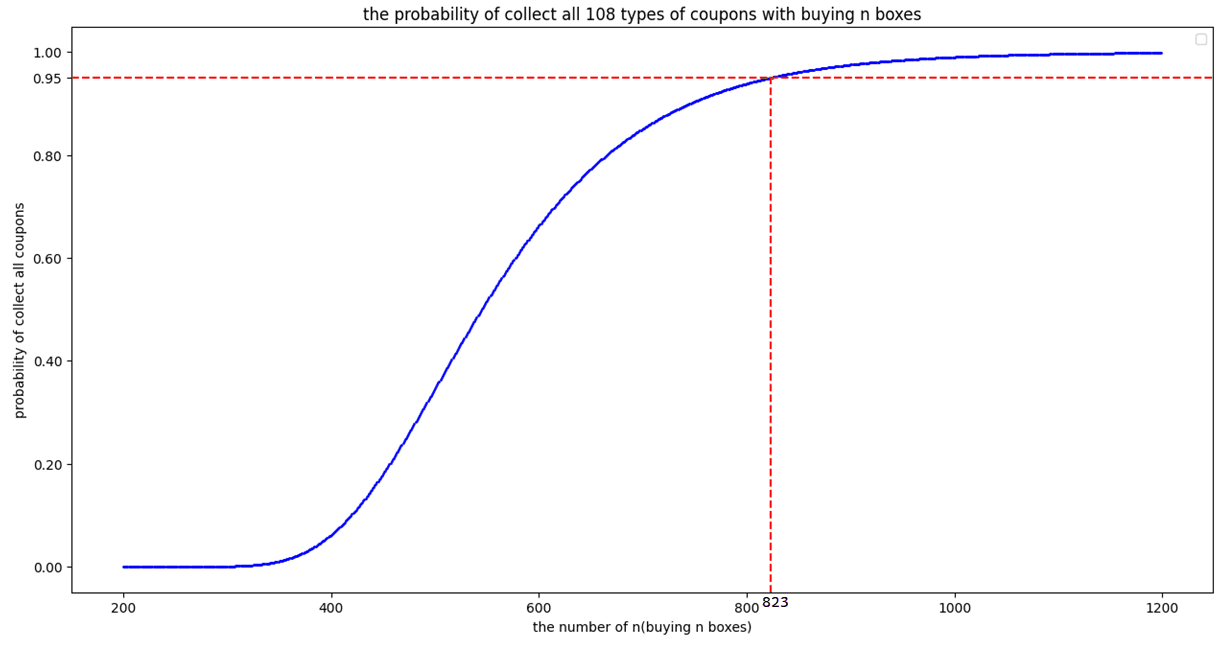
\includegraphics[width=1\linewidth]{q2}
    \caption{The probability of collect all 108 types of coupons with buying n boxes}
\end{figure}



\end{homeworkProblem}

\newpage


\begin{homeworkProblem}[3]

Since there are $100$ kits, and $5$ of them are defectives. So there are $95$ kits that are not defective.\\

So the total number of ways that we pick four of the kits with no defective, which means that the batch is 
accepted, is that we just pick $4$ in-defective kits from all $95$ in-defective kits. i.e. the number is ${95\choose 4}$.\\

And the number of all possible ways to pick kits is to pick $4$ kits from all $100$ kits. i.e. the number is ${100\choose 4}$.\\

$$P(the\ batch\ is\ accepted) = P(\dfrac{\# pick\ up\ four\ kits\ with\ no\ defective}{\# pick\ four\ kits\ from\ all\ kits})$$
$$= \dfrac{{95\choose 4}}{{100\choose 4}}$$
$$= \dfrac{\dfrac{95!}{4!(95-4)!}}{\dfrac{100!}{4!(100-4)!}}$$
$$= \dfrac{95*94*93*92}{100*99*98*97}$$
$$= \dfrac{76405080}{94109400}$$
$$\approx 0.811875$$

So above all, the possibility that the batch is accepted if it contains five defectives is $0.811875$.

\end{homeworkProblem}

\newpage

\begin{homeworkProblem}[4]
let $A_1$ : "the box that was chosen is box $a$"\\ 
let $A_2$ : "the box that was chosen is box $b$"\\
let $A_3$ : "the box that was chosen is box $c$"\\

And let $B$ : "the first coin that withdrew out is gold"\\
let $C$ : "the second coin that withdrew out is gold"\\

so $P(A_1) = P(A_2) = P(A_3) = \dfrac{1}{3}$, and $P(B|A_1) = 1,P(B|A_2) = 0,P(B|A_3) = \dfrac{1}{2}$\\
from LOTP, we could calculate that $$P(B) = \sum_{i = 1}^{3}P(B|A_i)P(A_i)$$ 
$$=P(B|A_1)P(A_1) + P(B|A_2)P(A_2) + P(B|A_3)P(A_3)$$
$$= 1*\dfrac{1}{3} + 0*\dfrac{1}{3} + \dfrac{1}{2}*\dfrac{1}{3}$$
$$ = \dfrac{1}{2}$$

And from the Bayes' Rule, we can calculate that $$P(A_1|B)=\dfrac{P(B|A_1)P(A_1)}{P(B)}$$
$$=\dfrac{1*\dfrac{1}{3}}{\dfrac{1}{2}}$$
$$=\dfrac{2}{3}$$

And since $P(C|B,A_1)=1,P(C|B,A_2)=0,P(C|B,A_3)=0$\\
from the LOPT with Extra Conditioning, we could calculate that
$$P(C|B)=\sum_{i=1}^{3}P(C|B,A_i)P(A_i|B)$$
$$=P(C|B,A_1)P(A_1|B) + P(C|B,A_2)P(A_2|B) + P(C|B,A_3)P(A_3|B)$$
$$=1*\dfrac{2}{3} + 0 + 0$$
$$=\dfrac{2}{3}$$

So above all, the probability of the coin drawn from the same bix also being a gold coin
is $P(C|B) = \dfrac{2}{3}$

\end{homeworkProblem}

\newpage

\begin{homeworkProblem}[5]
(a) If Mirana plays bold in both games $1$ and $2$. So for the first two games, there will have four different possibilities.\\
    \begin{itemize}
        \item Mirana wins all two games.\\
              With the possibility of $p_w^2$, she wins the match.
        \item Mirana wins first game and loses the second one.\\
              With the possibility of $p_w(1-p_w)$, she ties in the first two games.
        \item Mirana loses the first game and wins the second one.\\
              With the possibility of $(1-p_w)p_w$, she ties in the first two games.
        \item Mirana loses all two games.\\
              She losess the match.
    \end{itemize}    
    And we only consider about she wins the match, so for the second and the third situation, she has to win the third game, with the possibility of $p_w$.\\
    So above all, the possibility she wins the match is \\$P = p_w^2 + [p_w(1-p_w)+(1-p_w)p_w]p_w$\\
    $=3p_w^2-2p_w^3$\\

(b)  If Mirana plays timid in both games $1$ and $2$, the she will only tie or lose in the first two game.\\
from the rules, we know that if Mirana wins the match, then she has to tie on the first $2$ games, otherwise it is impossible for her to get into the third game.
So the possibility for her to get into the third game is $p_d^2$.\\
As she tie on the first two games, she plays bold on the third game, so her has the possibility of $p_w$ to win the third game, also win the match.\\
So above all, the possibility for her to win the match in this case is $P = p_d^2p_w$.\\

(c) Since the initial score is 0:0(regard Mirana is the prior number), so she has to play bold at the first game.
\begin{itemize}
    \item if she wins the first game, then the score is 1:0, so she will play timid in the second game.
        \begin{itemize}
            \item if she ties the second game, then the score is 1:0, and she wins the match with the possibility of $p_wp_d$.
            \item if she loses the second game, then the score is 1:1, and she will play bold in the third game.
                  So for this case, she will have the possibility of $p_w(1-p_d)p_w$ to win the match.
        \end{itemize}
    \item if she loses the first game, then the score is 0:1, so she will play bold in the second game.
        \begin{itemize}
            \item if she wins the second game, then the score is 1:1, and she will play bold in the third game.
            So for this case, she will have the possibility of $(1-p_w)p_w\cdot p_w$ to win the match.
            \item if she loses the second game, then the score is 0:2, and she loses the match.
        \end{itemize}
\end{itemize}

So above all, the possibility for her to win the match in this case is\\
$P = p_wp_d + p_w(1-p_d)p_w + (1-p_w)p_w\cdot p_w$\\
$=-p_w^3-p_w^2p_d+2p_w^2+p_wp_d$\\

(d) Let $P=-p_w^3-p_w^2p_d+2p_w^2+p_wp_d$\\
If we take $p_d = 1, p_w = 0.45$, then we could calculate that $P = 0.561375>\dfrac{1}{2}$\\
So Miriana may have a better than a $50-50$ chance to win the match.\\

$\dfrac{\partial P}{\partial p_d}=-p_w^2+p_w$\\
And since $0\leq p_w < \dfrac{1}{2}$, so $\dfrac{\partial P}{\partial p_d}\geq 0$\\
So for a given $p_w$, $P$ increases with the increase of $p_d$.\\
So for a given $p_w,P_{max} = P_{|p_d=1}=-p_w^3+p_w^2+p_w$.\\
Let $f(x)=-x^3+x^2+x$, then $f'(x)=-3x^2+2x+1=-(3x+1)(x-1)$,
so $f'(x)\geq 0$, for $0\leq p_w<\dfrac{1}{2}$,\\
so $f(x)$ increases with the increase of $x$.
And we could discover that $f(0.41)=0.509179>\dfrac{1}{2}$, from the continuity of function, we can know that there are many choices of $p_w,p_d$ to make $p > \dfrac{1}{2}$.\\

More intuitively, from the analysis in (c), we can see that when $p_w$ is close to $0.5$ and $p_d$ is close to $1$,
Marana can greatly maintain her advantage in the second game(which is $p_d$),if she wins the first game. That can make her win the match.\\
If she wins the first game but loses the second game, she still has $p_w$'s possibility to win the match.\\
And if she loses the first game, she still has $p_w^2$'s possibility to win the final match.\\
So if she win at first, she can greatly maintain the advantage, if she loses later, or loses at first, she still have chances to win.\\ 
So above all, when $p_w$ is close to $0.5$ and $p_d$ is close to $1$, although she is the worst player, she could 
greatly maintain her advantage, and try her best in disadvantage. So she may have a beeter than a $50-50$ chance to win the match.







\end{homeworkProblem}

\newpage

\end{document}
